%%%%%%%%%%%%%%%%%%%%%%%%%%%%%%%%%%%%%%%%%%%%%%%%%%%%%%%%%%%%%%%%%%%%%%%%%%%%%%%%%%%%%%%%%%%%%%%%%%%%%%%%%%%%%%%%%%%%%%%%%%%%%%%%%%%%%%%%%%%%%%%%%%%%%%%%%%%
% This is just an example/guide for you to refer to when producing your supplementary material for your Frontiers article.                                 %
%%%%%%%%%%%%%%%%%%%%%%%%%%%%%%%%%%%%%%%%%%%%%%%%%%%%%%%%%%%%%%%%%%%%%%%%%%%%%%%%%%%%%%%%%%%%%%%%%%%%%%%%%%%%%%%%%%%%%%%%%%%%%%%%%%%%%%%%%%%%%%%%%%%%%%%%%%%

%%% Version 2.5 Generated 2018/06/15 %%%
%%% You will need to have the following packages installed: datetime, fmtcount, etoolbox, fcprefix, which are normally inlcuded in WinEdt. %%%
%%% In http://www.ctan.org/ you can find the packages and how to install them, if necessary. %%%
%%%  NB logo1.jpg is required in the path in order to correctly compile front page header %%%

\documentclass[utf8]{frontiers_suppmat} % for all articles
\usepackage{url,hyperref,lineno,microtype}
\usepackage[onehalfspacing]{setspace}

\graphicspath{{figures/}}

\usepackage{xspace}

\newcommand{\insi}{\textit{in situ}\xspace}
\newcommand{\exsi}{\textit{ex situ}\xspace}
\newcommand{\apri}{\textit{a priori}\xspace}
\newcommand{\vivo}{\textit{in vivo}\xspace}
\newcommand{\vitro}{\textit{in vitro}\xspace}
\newcommand{\denovo}{\textit{de novo}\xspace}
\newcommand{\ie}{\textit{i.e.}\xspace}
\newcommand{\eg}{\textit{e.g.}\xspace}
\newcommand{\etc}{\textit{etc.}\xspace}
\newcommand{\vs}{\textit{vs.}\xspace}
\newcommand{\etl}{\textit{et al.}\xspace}
\newcommand{\perse}{\textit{per se}\xspace}

\newcommand{\rnaseq}{\textsc{RNA}-seq\xspace}
\newcommand{\scn}{\textsc{scNapBar}\xspace}
\newcommand{\scnast}{\textsc{scNaST}\xspace}

% Leave a blank line between paragraphs instead of using \\

\begin{document}
\onecolumn
\firstpage{1}

\title[Supplementary Material]{{\helveticaitalic{Supplementary Material}}}


\maketitle


%\section{Supplementary Data}
%
%Supplementary Material should be uploaded separately on submission. Please include any supplementary data, figures and/or tables. All supplementary files are deposited to FigShare for permanent storage and receive a DOI.
%
%Supplementary material is not typeset so please ensure that all information is clearly presented, the appropriate caption is included in the file and not in the manuscript, and that the style conforms to the rest of the article. To avoid discrepancies between the published article and the supplementary material, please do not add the title, author list, affiliations or correspondence in the supplementary files.

\section{Supplementary Tables and Figures}

\begin{figure}[htbp]
\begin{center}
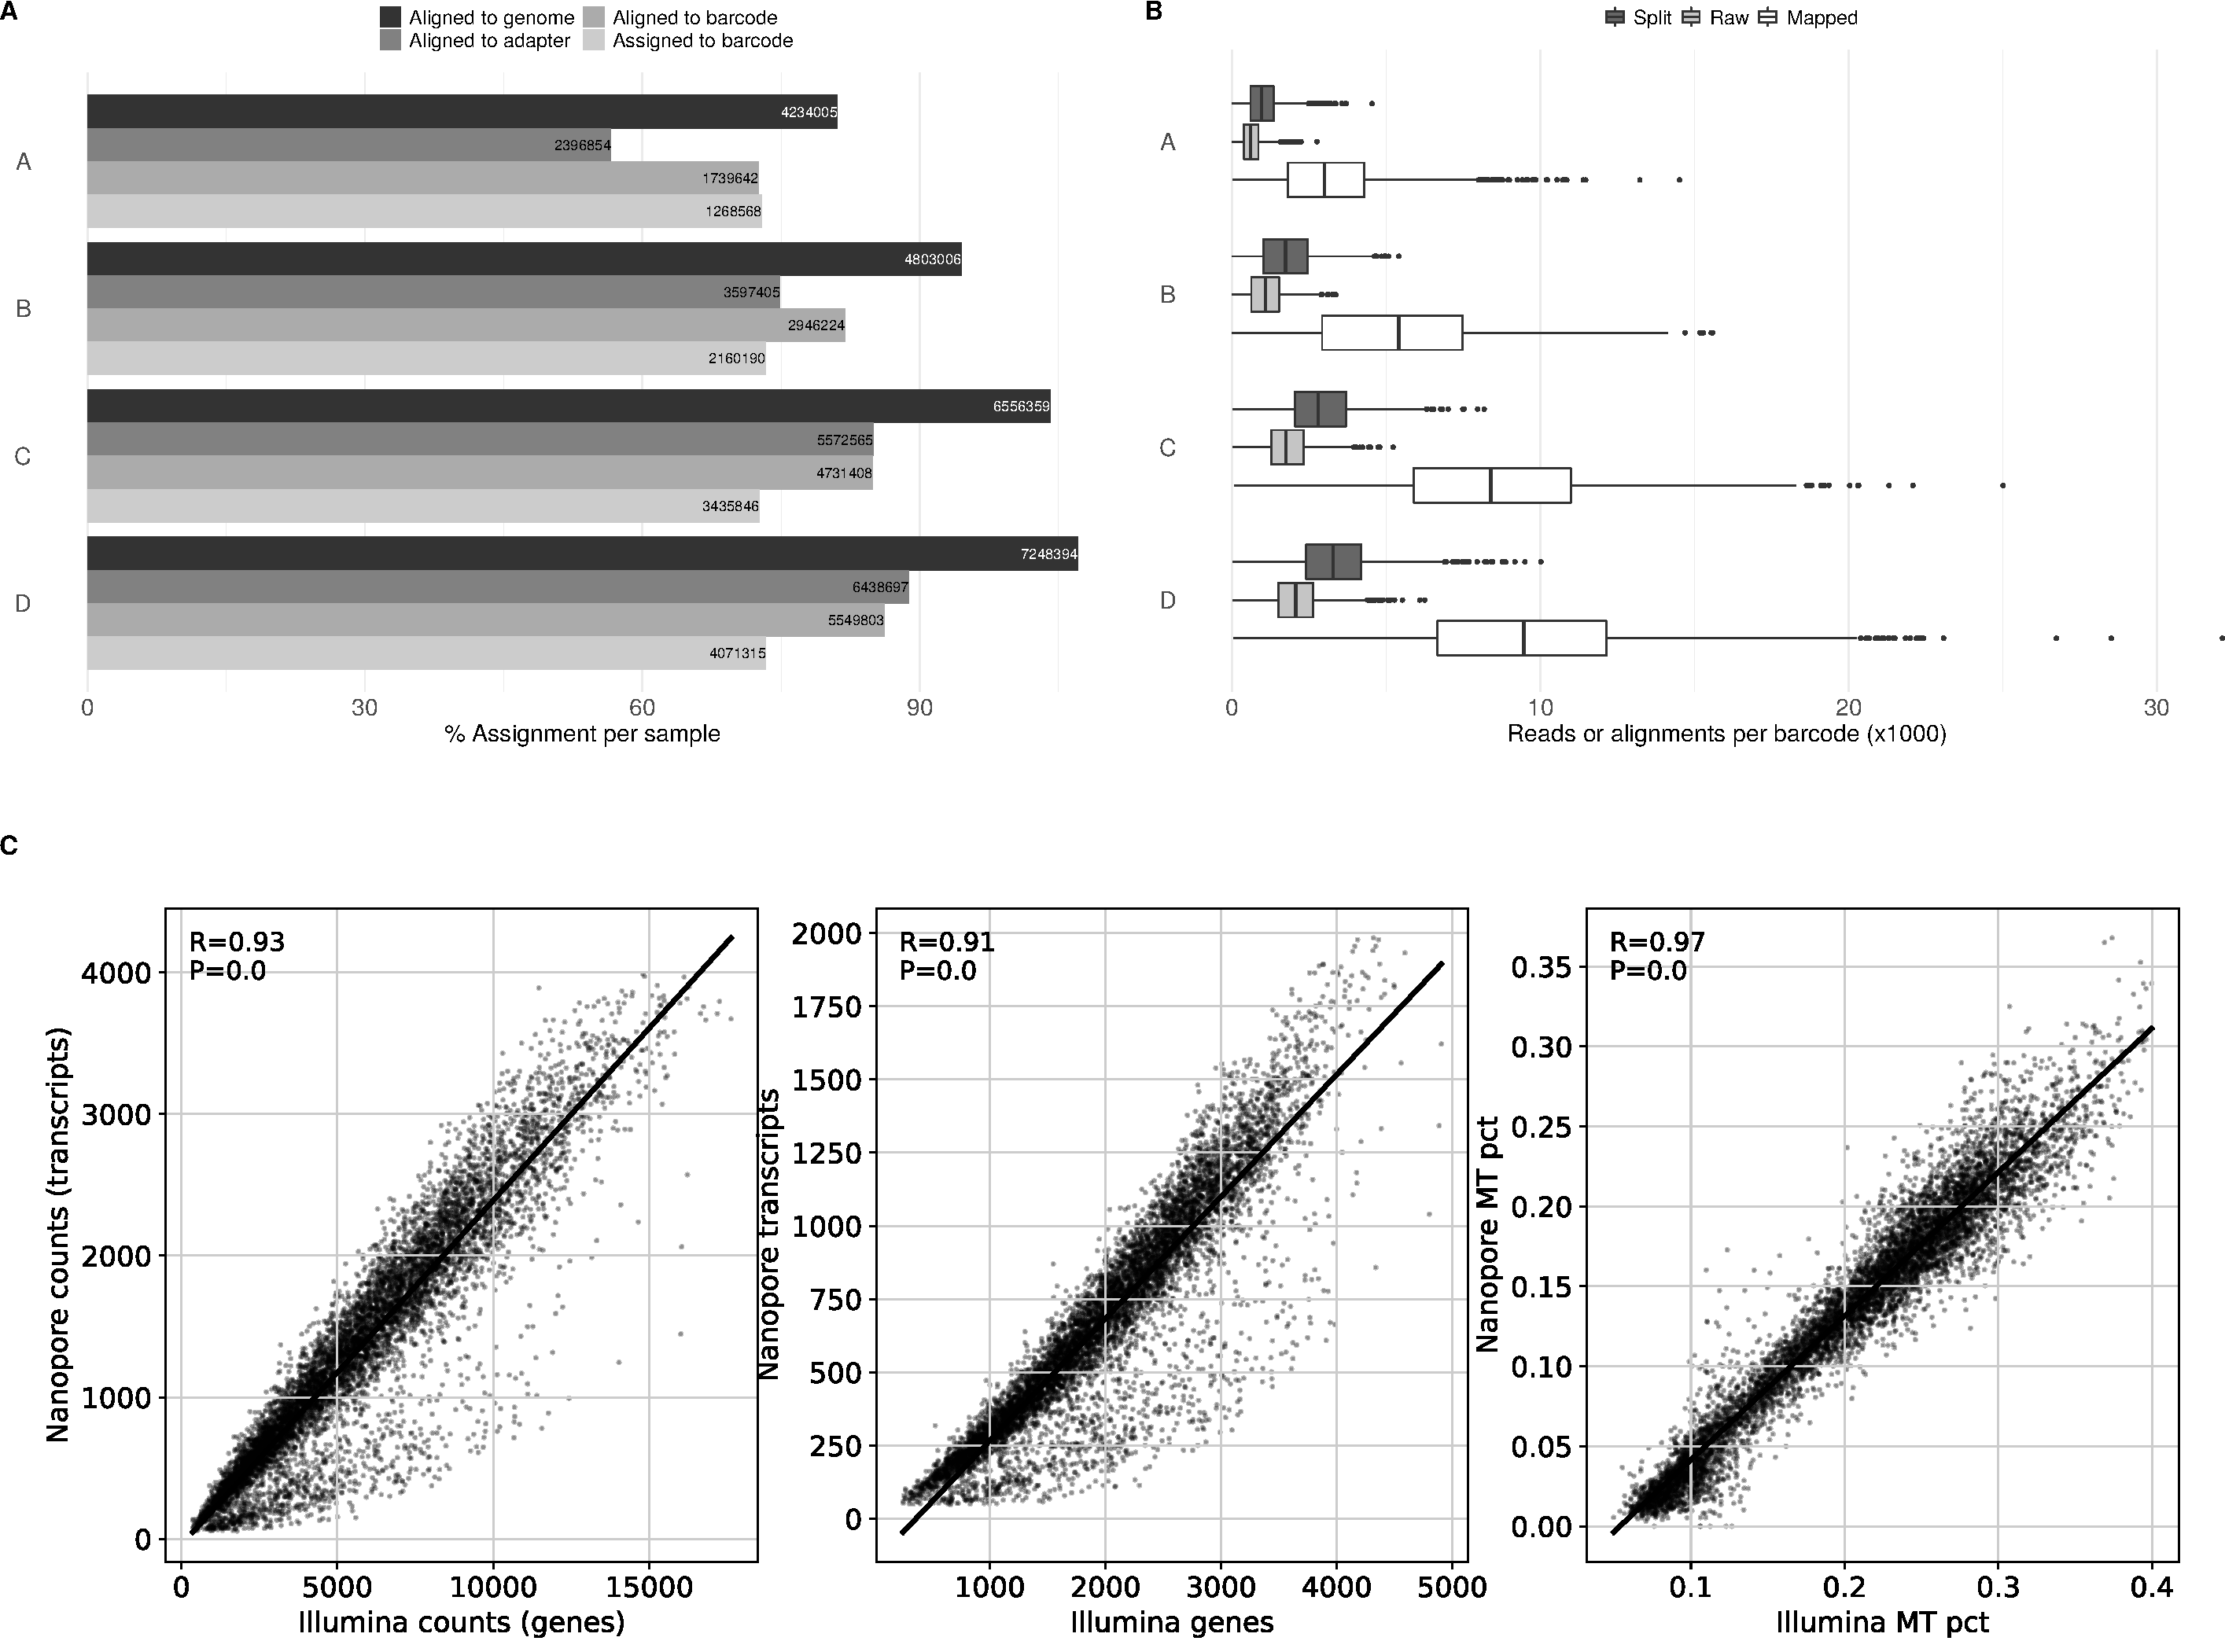
\includegraphics[width=\textwidth]{figS1}% This is a *.eps file
\end{center}
\caption{\scnast methodology. A Percentage of assignment by \scn at each step of the workflow for each heart slice (reads shown in bars). Reads aligned to genome are shown as a percentage of total reads. B Number of reads (or alignments) for each heart slice per spatial barcode. Split alignments are obtained from the genome mapped reads in \scn. Raw reads correspond to primary alignments converted to FASTQ format. Mapped are alignments to the transcriptome used for transcript abundance quantification. C Scatter plots showing the correlation between read counts, genes or transcripts, and the percentage of mitochondrial reads between Illumina and Nanopore libraries for all four samples, using the intersection of common spatial barcodes after quality filtering.}\label{fig:S1}
\end{figure}

\begin{figure}[htbp]
\begin{center}
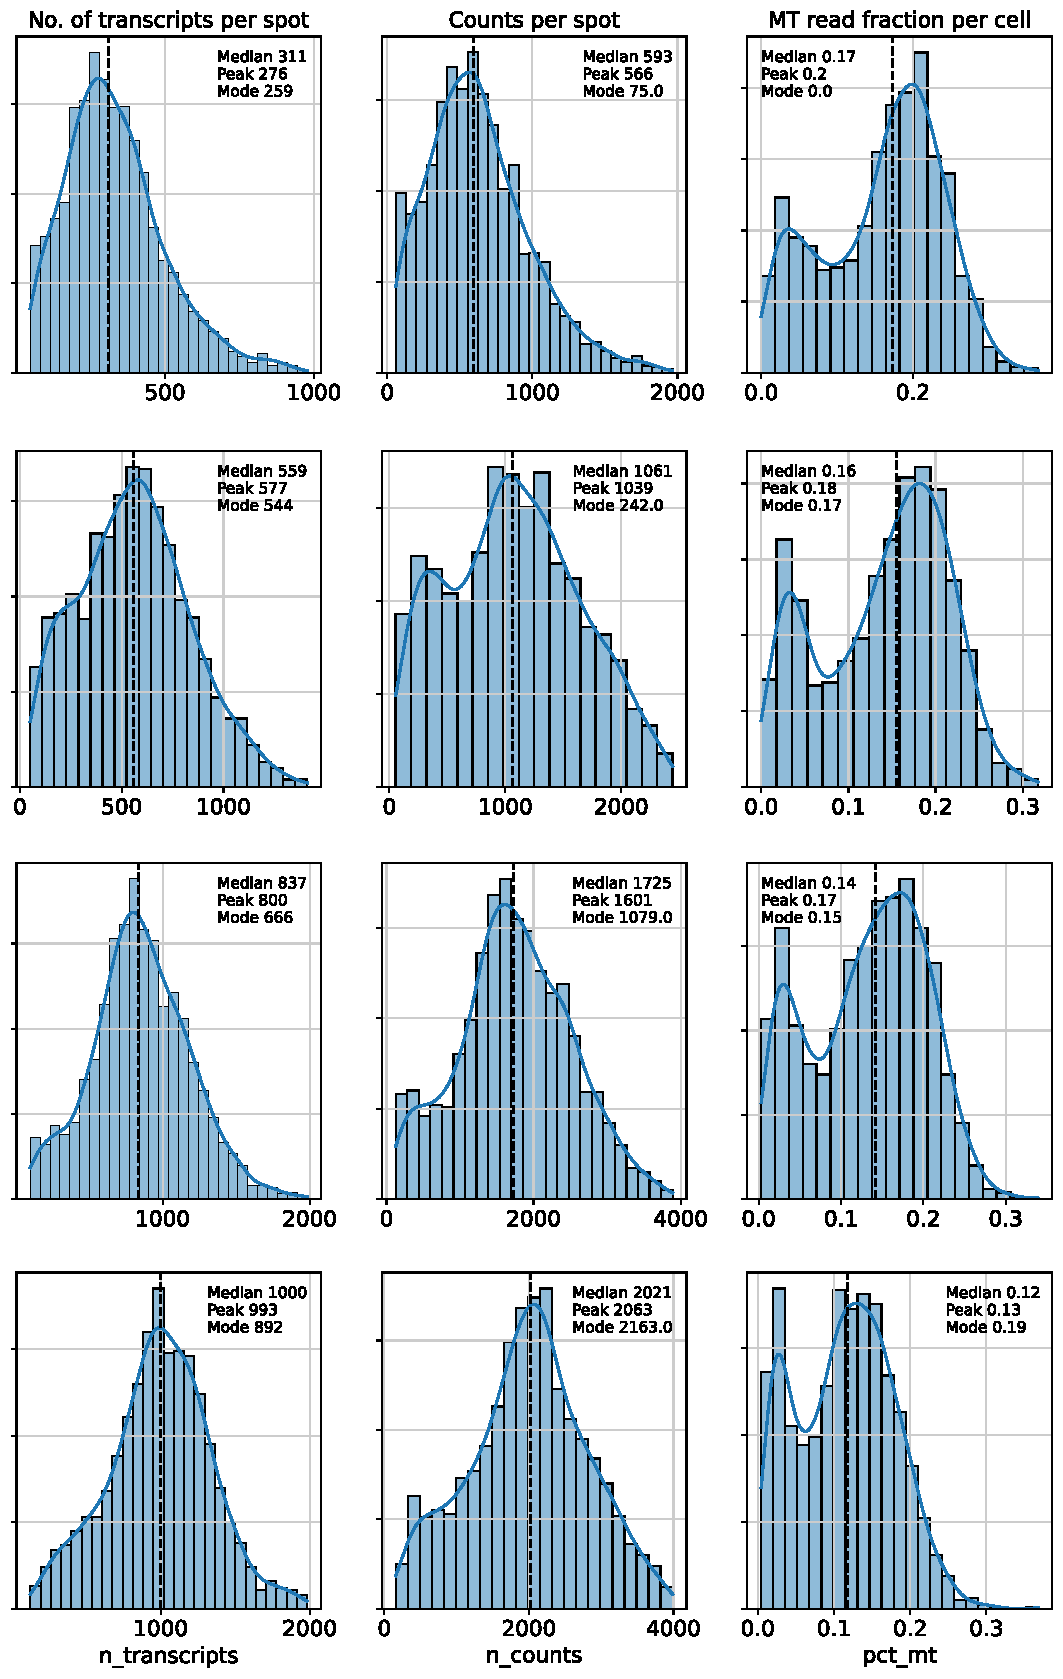
\includegraphics[width=.75\textwidth]{figS2}% This is a *.eps file
\end{center}
\caption{Quality control (Illumina). Distribution of number of genes, UMIs, and mitochondrial fraction per spatial spot after quality filtering, for each heart slice. From top to bottom: A, B, C, and D.}\label{fig:S2}
\end{figure}

\begin{figure}[htbp]
\begin{center}
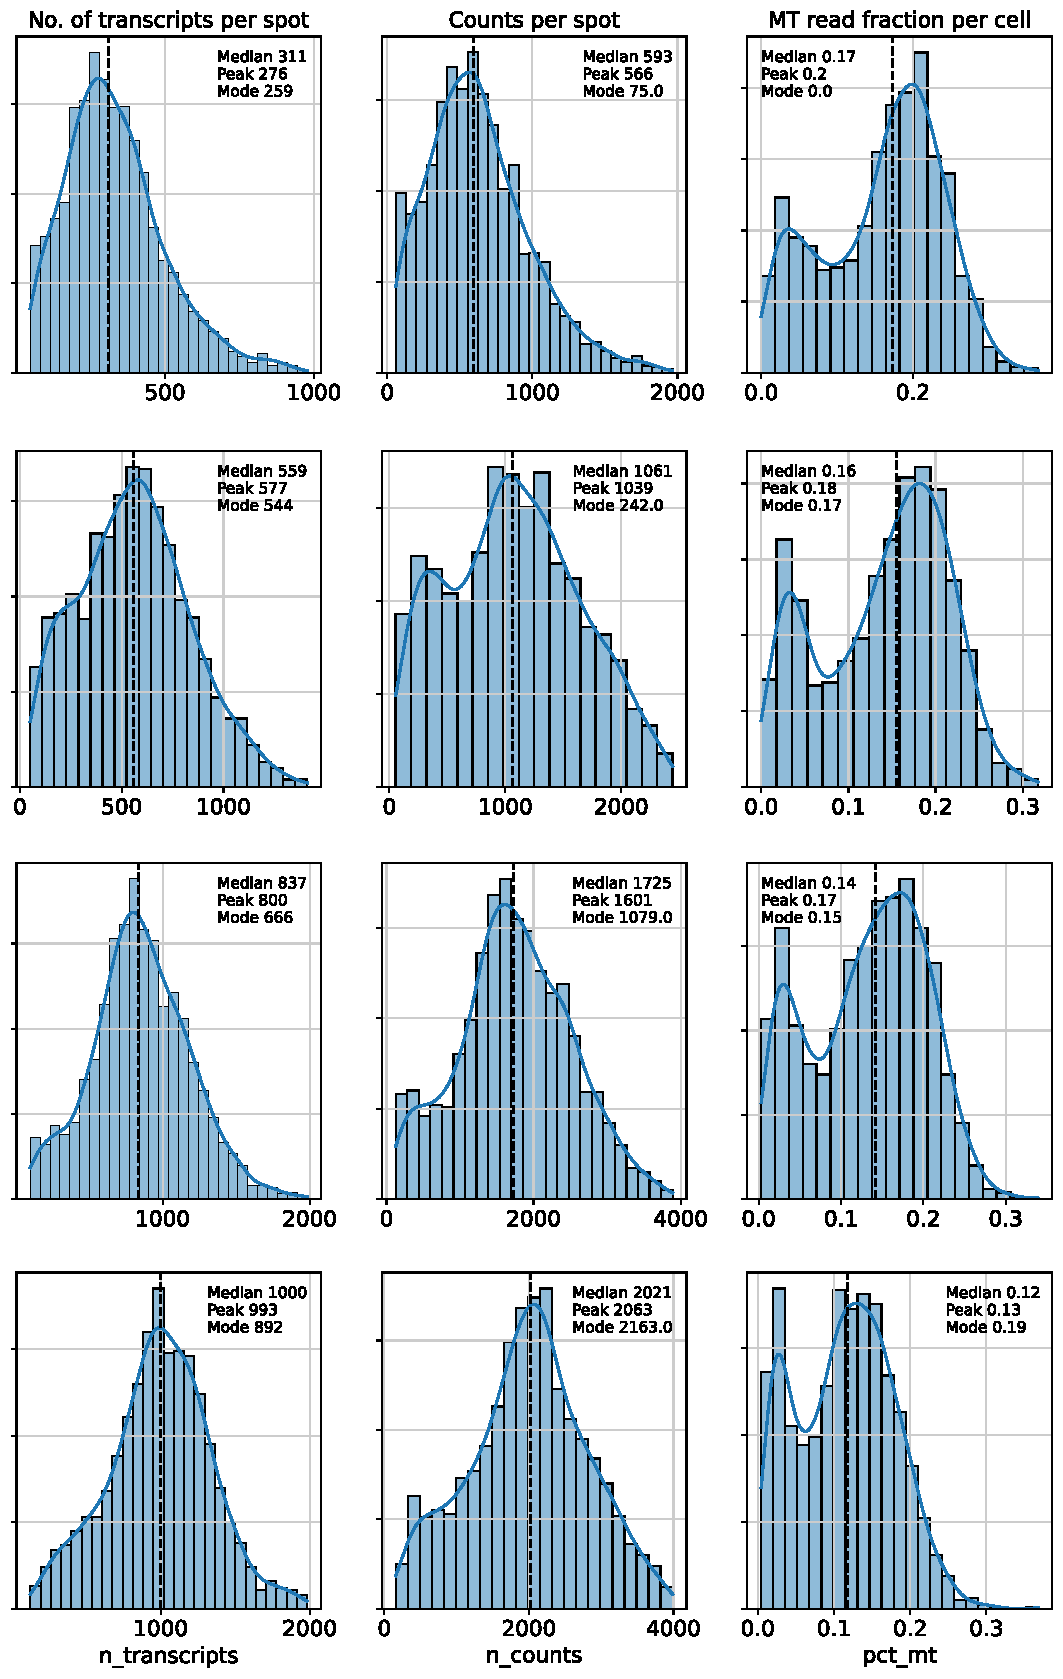
\includegraphics[width=.75\textwidth]{figS3}% This is a *.eps file
\end{center}
\caption{Quality control (Nanopore). Distribution of number of transcripts, counts, and mitochondrial fraction per spatial spot after assignment and quality filtering, for each heart slice. From top to bottom: A, B, C, and D.}\label{fig:S3}
\end{figure}


\begin{figure}[htbp]
\begin{center}
\includegraphics[width=\textwidth]{figS4}% This is a *.eps file
\end{center}
\caption{Spatial distribution of UMIs or counts (top) and genes or transcripts (bottom), for each A Illumina and B Nanopore libraries, for each heart slice (from left to right).}\label{fig:S4}
\end{figure}

\begin{figure}[htbp]
\begin{center}
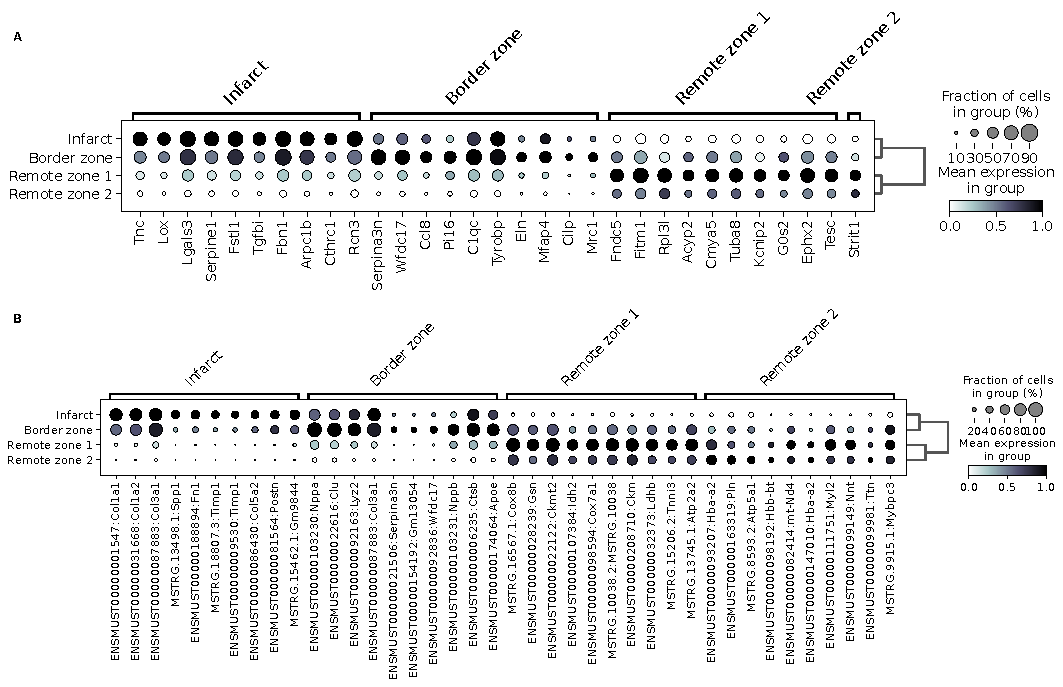
\includegraphics[width=\textwidth]{figS5}% This is a *.eps file
\end{center}
\caption{}\label{fig:S5}
\end{figure}

\begin{figure}[htbp]
\begin{center}
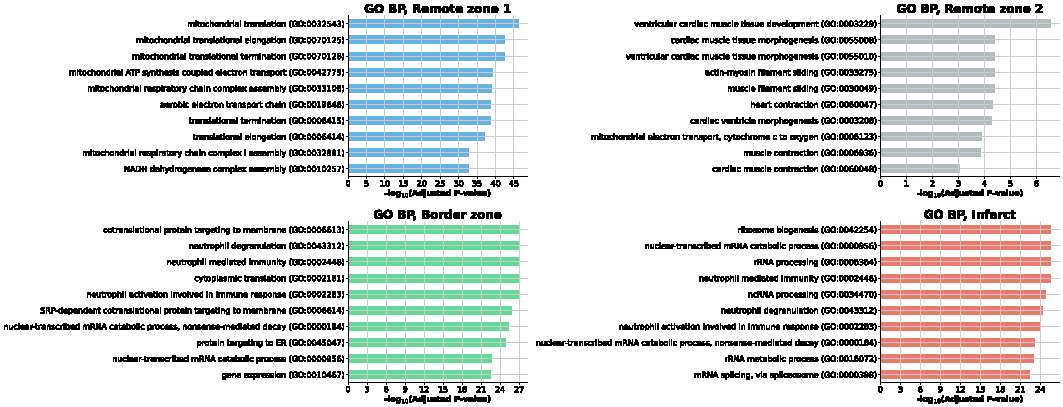
\includegraphics[width=\textwidth]{figS6}% This is a *.eps file
\end{center}
\caption{}\label{fig:S6}
\end{figure}

\begin{figure}[htbp]
\begin{center}
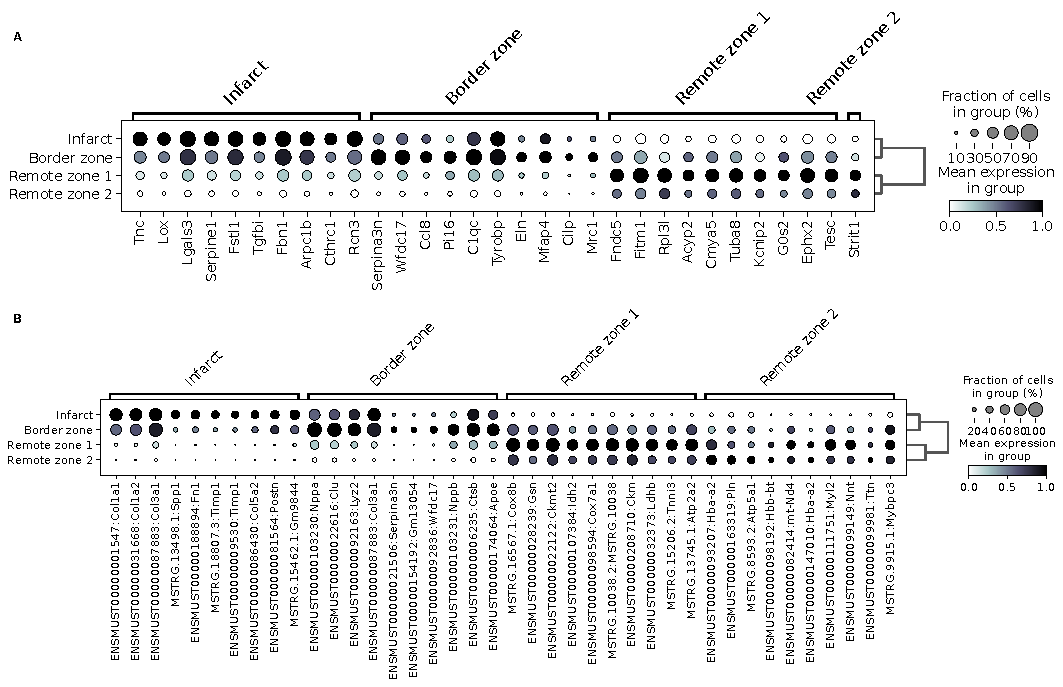
\includegraphics[width=\textwidth]{figS7}% This is a *.eps file
\end{center}
\caption{}\label{fig:S7}
\end{figure}

%\subsection{Figures}
%
%%%% There is no need for adding the file termination, as long as you indicate where the file is saved. In the examples below the files (logo1.eps and logos.eps) are in the Frontiers LaTeX folder
%%%% If using *.tif files convert them to .jpg or .png
%%%%  NB logo1.eps is required in the path in order to correctly compile front page header %%%
%
%\begin{figure}[htbp]
%\begin{center}
%
\includegraphics[width=9cm]{logo1}% This is a *.eps file
%\end{center}
%\caption{ Enter the caption for your figure here.  Repeat as  necessary for each of your figures}\label{fig:1}
%\end{figure}
%
%
%\begin{figure}[htbp]
%\begin{center}
%\includegraphics[width=10cm]{logos}
%\end{center}
%\caption{This is a figure with sub figures, \textbf{(A)} is one logo, \textbf{(B)} is a different logo.}\label{fig:2}
%\end{figure}

%%% If you are submitting a figure with subfigures please combine these into one image file with part labels integrated.
%%% If you don't add the figures in the LaTeX files, please upload them when submitting the article.
%%% Frontiers will add the figures at the end of the provisional pdf automatically
%%% The use of LaTeX coding to draw Diagrams/Figures/Structures should be avoided. They should be external callouts including graphics.


%\bibliographystyle{Frontiers-Harvard} %  Many Frontiers journals use the Harvard referencing system (Author-date), to find the style and resources for the journal you are submitting to see \href{https://zendesk.frontiersin.org/hc/en-us/articles/360017860337-Frontiers-Reference-Styles-by-Journal}{Frontiers Reference Styles by Journal}. For Humanities and Social Sciences articles please include page numbers in the in-text citations 
%\bibliographystyle{Frontiers-Vancouver} % Many Frontiers journals use the numbered referencing system, to find the style and resources for the journal you are submitting to see \href{https://zendesk.frontiersin.org/hc/en-us/articles/360017860337-Frontiers-Reference-Styles-by-Journal}{Frontiers Reference Styles by Journal}.

%\bibliography{test}

\end{document}
